\documentclass[a4paper, 12pt]{article}
% math symbols
\usepackage{amssymb}
\usepackage{amsmath}
\usepackage{mathrsfs}
\usepackage{physsummer}


\usepackage{enumitem}
\usepackage[margin = 2cm]{geometry}

\tolerance = 1000
\emergencystretch = 0.74cm



\pagestyle{empty}
\parindent = 0mm

\begin{document}

\begin{center}
  \Large{\textbf{11 класс.}\\
  \textit{12 ноября 2014.}}
\end{center}


\begin{center}
  \Large \textbf{ Геометрическая оптика.}
\end{center}

\large

\taskpic{ Высокий цилиндрический стакан плавает в жидкости плотностью
  $\rho$. На дне стакана лежит вогнутое зеркало с радиусом кривизны
  $R$; оптическая ось зеркала совпадает с осью стакана. На высоте $H$
  над поверхностью жидкости строго над серединой стакана расположена
  лампочка. При какой суммарной массе стакана и зеркала в нём
  изображение лампочки окажется на уровне поверхности жидкости? Радиус
  дна стакана $r$. }
{
  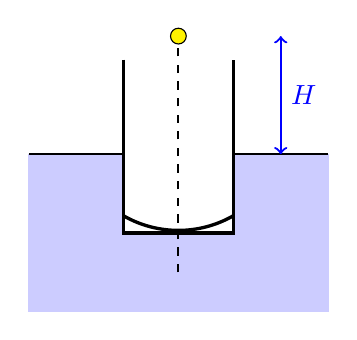
\begin{tikzpicture}
    \draw[fill=blue!20,draw=blue!20] (0,0) rectangle (3.8,-2);
    \draw[thick] (0,0) -- (3.8,0);
    \draw[fill=white,draw=white] (1.2,1.5) rectangle (2.6,-1);
    \draw[very thick] (1.2,1.2) -- (1.2,-1) -- (2.6,-1) -- (2.6,1.2);
    \draw[very thick] (1.2,-0.78) arc (240:300:1.4cm);
    \draw[dashed,thick] (1.9,-1.5) -- ++ (0,3);
    \draw[fill=yellow] (1.9,1.5) circle (0.1cm);
    \draw[blue,<->,thick] (3.2,0) -- (3.2,1.5) node[midway,right]
    {$H$}; 
  \end{tikzpicture}
}
% СПб, район-11, 2014

\task{ Параллельно главной оптической оси собирающей линзы с фокусным
  расстоянием $F$ движется точечный источник света. На каком
  расстоянии от линзы он окажется в тот момент, когда скорость его
  изображения в линзе будет равна по величине скорости источника?
  Расстояние от главной оптической оси линзы до источника $H=F$. }
% Зильберман, ШФО, стр. 182

\task{ На расстоянии $d=0.6$ см от центра стеклянного шара радиуса
  $R=1$ см находится точечный источник света. При каких значениях
  коэффициента преломления стекла $n$ весь испускаемый источником
  световой поток выйдет наружу? Снаружи --- вакуум, источник излучает
  во все стороны равномерно. }
% Зильберман, ШФО, стр. 182

\task{ Два плоских зеркала образуют двугранный угол, равны
  $\pi/2$. Собирающая линза с фокусным расстоянием $F$ вставлена в
  угол так, что её главная оптическая ось составляет угол $\pi/4$ с
  каждым зеркалом. Диаметр линзы равен $2F$. На главной оптической оси
  линзы на расстоянии $d=1.5F$ от линзы находится источник света
  $S$. Найдите положение изображения источника света. }
% Туймада, 4.1

\taskpic{ С помощью системы концентрических зеркал на экране получено
  изображение Солнца. Радиусы зеркал $R_1 = 12$ см, $R_2 = 30$
  см. Каково должно быть фокусное расстояние тонкой линзы, чтобы с её
  помощью получалось изображение Солнца такого же размера? }
{
\begin{tikzpicture}
  \draw[thick,interface] ({3+cos(110)},{2+sin(110)}) arc (110:250:1);
  \draw[thick,interface] ({3+1.5*cos(160)},{2+1.5*sin(160)}) arc
  (160:110:1.5);
  \draw[thick,interface] ({3+1.5*cos(250)},{2+1.5*sin(250)}) arc
  (250:200:1.5);
  \draw[thick,->] (0,2) -- (1.2,2);
  \draw[thick,->] (0,2.4) -- (1.2,2.4);
  \draw[thick,->] (0,1.6) -- (1.2,1.6);
  \draw[blue,->] (3,2) -- ({3+cos(140)},{2+sin(140)}) node[near
  start,above] {$R_1$};
  \draw[blue,->] (3,2) -- ({3+1.5*cos(220)},{2+1.5*sin(220)})
  node[near start,below] {$R_2$};
\end{tikzpicture}
}
% Квант, 1981-09, Ф677

\end{document}


%%% Local Variables: 
%%% mode: latex
%%% TeX-engine:xetex
%%% TeX-PDF-mode: t
%%% End:
